% cube with space diagonal BD1 and transversal MN (faithful to original PNG)
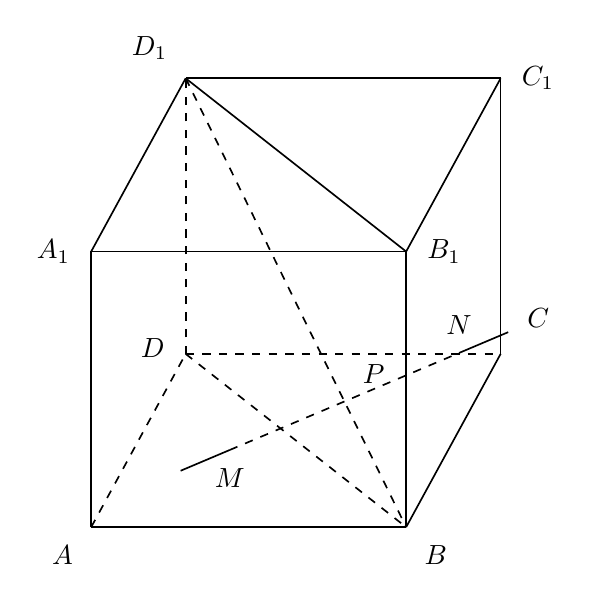
\begin{tikzpicture}[x=1cm,y=1cm,line width=.6pt,font=\normalsize]
\coordinate (A) at (0,0);
\coordinate (B) at (4,0);
\coordinate (C) at (5.2,2.2);
\coordinate (D) at (1.2,2.2);
\coordinate (Aone) at (0,3.5);
\coordinate (Bone) at (4,3.5);
\coordinate (Cone) at (5.2,5.7);
\coordinate (Done) at (1.2,5.7);
\coordinate (Lleft) at (1.1360000000,0.7160000000);
\coordinate (Lright) at (5.2960000000,2.4760000000);
\coordinate (Ppt) at (3.2160000000,1.5960000000);
% hidden bottom / interior (dashed)
\draw[dashed] (D) -- (C);
\draw[dashed] (A) -- (D);
\draw[dashed] (D) -- (Done);
\draw[dashed] (D) -- (B);
\draw[dashed] (Done) -- (B);
% transversal MN extended beyond cube (passes through A, P on BD1)
\coordinate (Mpt) at (1.76,0.9800000000000002);
\coordinate (Npt) at (4.672000000000001,2.2120000000000006);
\draw (Lleft)--(Mpt);
\draw[dashed] (Mpt)--(Npt);
\draw (Npt)--(Lright);
% visible cube outline
\draw (A) -- (B);
\draw (B) -- (C);
\draw (Cone) -- (Done);
\draw (Bone) -- (Cone);
\draw (A) -- (Aone) -- (Bone) -- (B);
\draw (Aone) -- (Done);
\draw (Bone) -- (Done);
\draw (C)--(Cone);
% labels offset to avoid touching strokes
\node[below left,xshift=-3pt,yshift=-3pt] at (A) {$A$};
\node[below right,xshift=3pt,yshift=-3pt] at (B) {$B$};
\node[above right,xshift=6pt,yshift=6pt] at (C) {$C$};
\node[left,xshift=-4pt,yshift=2pt] at (D) {$D$};
\node[left,xshift=-4pt] at (Aone) {$A_{1}$};
\node[right,xshift=4pt] at (Bone) {$B_{1}$};
\node[right,xshift=4pt] at (Cone) {$C_{1}$};
\node[above left,xshift=-3pt,yshift=3pt] at (Done) {$D_{1}$};
\node[below=3pt] at (1.7600000000,0.9800000000) {$M$};
\node[above=3pt] at (4.6720000000,2.2120000000) {$N$};
\node[above right,xshift=3pt,yshift=3pt] at (Ppt) {$P$};
\end{tikzpicture}
